 \appendix
 
\section{NP-completeness Proof of Enforcing Isolation Policies} \label{sec:isolationNP}
 We show that the graph 3-coloring problem, which is NP-complete reduces to the enforcement problem for
 reachability and isolation policies. The latter is also in NP, so after the reduction we 
 can conclude that it is also NP-complete.

Let $G=(V,E)$ be an instance of the graph 3-coloring problem.
The graph $G$ admits a 3-coloring if there exists a function 
$f:G\mapsto \{R,G,B\}$ such that for every edge $(v1,v2)\in E$,
$f(v_1)\neq f(v_2)$.

We now show how to construct a topology $T=(S,L)$ and a corresponding set of policies $P$ that can be 
enforced iff $G$ admits 3-coloring.
The topology $T$ is the one depicted in  \Cref{fig:swtopo}.
The set of flows is $V$, $v \in V$ we add a reachability policy $s >> d$ on the flow $v$.
For each edge $(v1,v2)\in E$ we add an isolation policy $v_1||v_2$.
% \begin{figure}[H] 
% 	\centering
% 	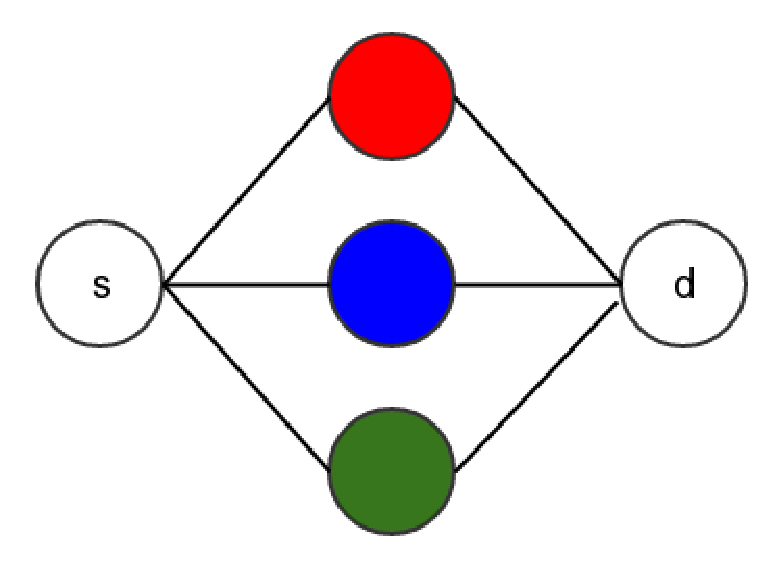
\includegraphics[width=0.5\columnwidth]{figures/color_topo.eps}
% 	\caption{The switch topology $T$. All circles represent switches and all reachability policies are $s$ to $d$}
% 	\label{fig:swtopo}
% \end{figure}
\begin{figure}[h!]
	\centering
	\begin{tikzpicture}[shorten >=0.5pt,node distance=1.5cm,on grid,auto] 
	\node[state] (s)   {$s$}; 
	\node[state, fill=black!10!red] (r) [right=of s] {}; 
	\node[state, fill=white!30!blue] (b) [above=of r] {};
	\node[state, fill=black!30!green] (g) [below=of r] {}; 
	\node[state] (d) [right=of r] {$d$}; 	
	\path[-] 
	(s) edge  node {} (r)
	edge node {} (b)
	edge node {} (g)
	(r) edge node {} (d)
	(g) edge node {} (d)
	(b) edge node {} (d);
	\end{tikzpicture}
	\caption{The switch topology $T$. All circles represent switches and all reachability policies are $s$ to $d$}
	\label{fig:swtopo}
\end{figure}
We now prove that if the policies can enforced then $G$ admits 3-coloring.
If the policy is enforced, we have a path from $s$ to $d$ for each flow/vertex $v$.
We can set $f(v)$ to the color of the corresponding middle-switch being crossed.
Since for every $(v1,v2)\in E$ the two flows for $v_1$ and $v_2$ cannot share any edge,
they must have crossed two middle-switches with different colors and $f$ is a correct 3-coloring.
The other direction of the proof is analogous.

 
% \subsection{Enforcement of Waypoint Policies}
% Given a undirected graph $G={V,E}$. Let us assume there exists an polynomial-time algorithm to compute the reachability paths satisfying the policies of the following types on the graph : \\
% \begin{itemize} 
% 	\item \textbf{P1} : $v_1 >> v_2 \Rightarrow$ There exists a path from $v_1$ to $v_2$ satisfying all input policies. A property of the path is that it does not have repeat a vertex (no forwarding loops).
% 	\item \textbf{P2} : $v_1 >> W >> v_2 \Rightarrow$ The path from $v_1$ to $v_2$  should pass through the vertices in the set $W$ in any order, without repeating a vertex.
% \end{itemize}
% \textbf{Reduction of Hamiltonian Cycle Problem} : Given a undirected graph $G={V,E}$, find $v \in V$ such that the degree of $v$ is the minimum in the graph (Will work for any vertex actually). If a Hamiltonian cycle is present in the graph, it will have the vertex $v$ in the cycle, and one of the edges from $v$.  \\
% Lets take a $n \in Neighbours(v)$. Let the input policies to our algorithm be : 
% \begin{itemize}
% 	\item \textbf{P4} : $v >> W >> n$ where $W = V - \{v,n\} $ 
% \end{itemize}
%P4 cimputes a simple path from $v$ to $n$ which passes through all the other vertices in the graph which is the Hamiltonian path problem. Since computing the Hamiltonian path is NP-hard, the problem of path computation for the waypoint policies as specified is NP-hard. 
\section{Tactics}
\begin{theorem}[Soundness]
	For a tactic R, if $(Fwd, Reach) \models \Psi \wedge \Psi_R$, then $\forall (\pi, pc) \in \Pi. \ \pi \models_{pc} R$.
\end{theorem}
\begin{proof}
	The proof of this theorem is by contradiction for each type of tactic. \newline
	\textbf{Type 1}: R = $\neg (l_{src} .^i .^* l_{dst})$ \\
	%$\forall sw,k \geq i + 1. (sw,pc,k) \notin Reach \implies \pi \models \neg (l_{src} .^i .^* l_{dst}) $ \newline
	\textbf{Assume  $\pi \not\models R$}.  $\pi \models l_{src} .^i .^* l_{dst}$. \\
	Thus, $\pi = src\ sw_1 \ldots sw_i \ldots dst$. \\
	Therefore,  $(dst, pc, k_{dst}) \in Reach, k_{dst} \geq i + 1$. \\
	However, $\pi \models_{pc} \Psi_R \Leftrightarrow \pi \models_{pc} \forall sw,k \geq i + 1. (sw,pc,k) \notin Reach$.
	Contradiction, as $\exists sw, k \geq i + 1. (sw,pc,k) \in Reach$.
	\newline
	\newline
	\textbf{Type 2}: $R = \neg (l_{src} .^i \ l \ .^* l_{dst})$ \newline
	\textbf{Assume  $\pi \not\models R$}. $\pi \models l_{src} .^i \ l \ .^* l_{dst}$. \\
	Thus, $\pi = src\ sw_1 \ldots sw_i \ sw_{i+1} \ldots dst$ such that $\phi(sw_{i+1}) = l$. Also $sw_{i+1} \not=dst$ (dst has to be the last switch in $\pi$)\\
	Therefore,  $(sw_{i+1}, pc, i+1) \in Reach$. \\
	However,
	$\pi \models_{pc} \Psi_R \Leftrightarrow \pi \models_{pc}\forall sw.~ \phi(sw) = l ~\wedge~ sw \not= dst \implies  (sw, pc, i + 1) \notin Reach$. \\
	Contradiction, as $\exists sw. ~ \phi(sw) = l ~\wedge~ sw \not= dst \wedge (sw,pc,i+1) \in Reach$.
	\newline \newline
	\textbf{Type 3}: $R = \neg (l_{src} .^i \ l_1 \ l_2 \ .^* l_{dst})$ \newline
	\textbf{Assume  $\pi \not\models R$}. $\pi \models l_{src} .^i \ l_1 \ l_2 \ .^* l_{dst}$. \\
	Thus, $\pi = src\ sw_1 \ldots sw_i \ sw_{i+1} \ sw_{i+2} \ldots dst$ such that $\phi(sw_{i+1}) = l_1, \phi(sw_{i+2}) = l_2$. Also $sw_{i+2} \not=dst$ (dst has to be the last switch in $\pi$)\\
	Therefore,  $(sw_{i+1}, pc, i+1) \in Reach \wedge (sw_{i+1}, sw_{i+2}, pc) \in Fwd$. \\
	However,
	$\pi \models_{pc} \Psi_R \Leftrightarrow \pi \models_{pc} \forall n_1, n_2.~\phi(n_1) = l_1~\wedge~ \phi(n_2) = l_2 ~\wedge~ n_2 \not=dst  \implies 
	\neg (Reach(n_1, pc, i + 1) \wedge Fwd(n_1, n_2, pc))$. \\
	Contradiction, as $\exists n_1. n_2. ~\phi(n_1) = l_1~\wedge~ \phi(n_2) = l_2 ~\wedge~ n_2 \not=dst \wedge Reach(n_1, pc, i + 1) \wedge Fwd(n_1, n_2, pc)$. 
\end{proof}
\begin{theorem}[Completeness]
For a tactic R, if $~\Pi \models \Psi ~\wedge~$ $(\forall (\pi, pc) \in \Pi.~ \pi \models_{pc} R)$, then $(Fwd, Reach) \models \Psi_R$.
\end{theorem}
\begin{proof}
	The proof of this theorem is by contradiction for each type of tactic. \newline
	\textbf{Type 1}: $R = \neg (l_{src} .^i .^* l_{dst})$ \newline
	\textbf{Assume $\pi \not\models_{pc} \Psi_R$}. $\pi \not\models_{pc} \forall sw,k \geq i + 1. (sw,pc,k) \notin Reach$ \newline
	Therefore $\exists sw, k \geq i + 1. (sw,pc,k) \in Reach$. \\
	Therefore, $\pi \models l_{src}\ .^i \ .^* \ \phi(sw) \ .^* \ l_{dst} \implies \pi \models l_{src} .^i .^* l_{dst}$
	Contradiction, as $\pi \models R$.
	\newline 
	\newline 
	\textbf{Type 2}: $R = \neg (l_{src} .^i \ l \ .^* l_{dst})$ \newline
	\textbf{Assume  $\pi \not\models_{pc} \Psi_R$}.  $\pi \not\models_{pc}\forall sw.~ \phi(sw) = l ~\wedge~ sw \not= dst \implies  (sw, pc, i + 1) \notin Reach$. \\
	Therefore $\exists sw. \ sw \not= dst \ \wedge \ \phi(sw) = l \ \wedge \ (sw,pc,i+1) \in Reach$. \\
	Therefore, $\pi \models l_{src}\ .^i \ l \ .^* \ l_{dst}$. \\
	Contradiction, as $\pi \models R$. 
	\newline  
	\newline
	\textbf{Type 3}: $R = \neg (l_{src} .^i \ l_1 \ l_2 \ .^* l_{dst})$ \newline
	\textbf{Assume  $\pi \not\models_{pc} \Psi_R$}.  $\pi \not\models_{pc} \forall n_1, n_2.~\phi(n_1) = l_1~\wedge~ \phi(n_2) = l_2 ~\wedge~ n_2 \not=dst  \implies 
	\neg (Reach(n_1, pc, i + 1) \wedge Fwd(n_1, n_2, pc))$. 
	Therefore $\exists n_1, n_2. ~\phi(n_1) = l_1~\wedge~ \phi(n_2) = l_2 ~\wedge~ n_2 \not=dst ~\wedge~ Reach(n_1, pc, i + 1) ~\wedge~ Fwd(n_1, n_2, pc)$. \\
	Therefore, $\pi \models l_{src}\ .^i \ l_1~l_2 \ .^* \ l_{dst}$. \\
	Contradiction, as $\pi \models R$.
\end{proof}